\documentclass[conference]{IEEEtran}
\usepackage{cite}
\usepackage{amsmath,amssymb,amsfonts}
\usepackage{algorithmic}
\usepackage{graphicx}
\usepackage{textcomp}
\usepackage{xcolor}

\def\BibTeX{{\rm B\kern-.05em{\sc i\kern-.025em b}\kern-.08em
    T\kern-.1667em\lower.7ex\hbox{E}\kern-.125emX}}

\begin{document}

\title{Stock Market Price Prediction}

\author{\IEEEauthorblockN{Valliappan Chidambaram}
    \IEEEauthorblockA{\textit{Utah State University} \\
        Logan, UT, USA \\
        a02349758@aggies.usu.edu}}

\maketitle

\begin{abstract}
    Predicting stock market prices is fundamental to any investment strategy, as to make profits, one must sell a stock at a higher price than they bought it. Most traditional methods for forecasting the performance of a stock focus on long-term growth using things like a company's financial statements, though these are significantly less useful in the short-term, as short-term performance is highly noisy and volatile, dominated by things like news and investor behavior. This paper explores the possibility of using machine learning, particularly neural networks, to predict the price of stocks in the short term.
\end{abstract}

\section{Introduction}
The stock market presents an opportunity to make large amounts of profits with relatively minimal efforts, but it's also highly competitive and can often lead to losing equally large amounts of money. Many large companies, such as banks and investment firms, try to accumulate money by investing in the stock market. Traditional methods usually involve looking at aspects of a company's financial statements, like their earnings per share and debt, to predict how the stock will perform over a long period of time, and then buying stocks based on their predicted long-term performance. More recently, with the advent of machine learning, much research has been done to create models to predict stock prices over shorter time periods or select portfolios that are likely to perform well. Investors and companies often use these models to augment their decision-making process when buying stocks or use them outright when performing tasks like high frequency trading. Machine learning models for stock price prediction can also be useful because they lower the amount of domain knowledge required to make profitable decisions.

The stock market is extremely noisy and volatile, with stock prices fluctuating rapidly over time from a variety of external factors, ranging from investors buying and selling a stock over the course of a day to larger events like COVID-19 \cite{Ruan_2020} or news about specific companies. Most time-series forecasting methods, such as ARIMA, perform worse when the data being fit is noisy, though it is possible to work around this with methods like smoothing the data via interpolation methods \cite{yu2023application}. Neural networks, however, are much better at handling noisy inputs and outputs \cite{rolnick2018deep}, and recurrent neural networks such as long-short term memory (LSTM) networks can even be used solely to reduce noise \cite{9483103}. This paper explores the use of neural networks, including both convolutional neural networks (CNNs) and LSTMs, to forecast stock prices.

\section{Method}
\subsection{Dataset}
The dataset for these experiments was collected using NASDAQ's historical stock price API, which tracks the last 10 years of stock data for most stocks on their exchange. Data was collected for the largest 1000 stocks on the exchange by market cap, as large companies tend to have slightly more stable stock prices than smaller ones, and models trained on large-cap stocks were likely to generalize better to other large-cap stocks than to mid-cap or small-cap stocks. Additionally, the last 10 years of data was downloaded for the NASDAQ Composite index (COMP) and the Dow Jones Industrial Average index (DJIA), as data about overall stock market trends seemed likely to improve model performance. The data downloaded from the NASDAQ API included the opening price, closing price, high price, low price, and date for each day in the last 10 years. For stocks, but not indexes, the volume of shares traded was also included. The dataset was split into training, validation, and test sets by stock with a 60-20-20\% split. The dataset was split by stock instead of time period to limit the effect of anomalous events such as COVID-19 on model generalization.

\begin{figure}
    \centering
    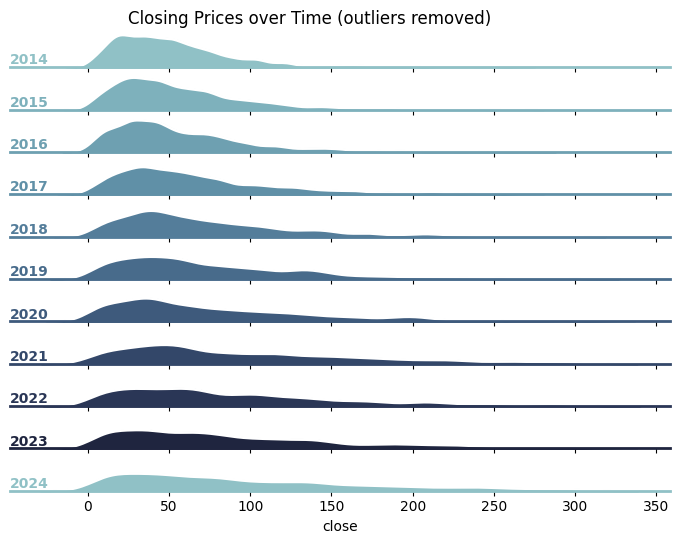
\includegraphics[width=\columnwidth]{figures/closeOverTime.png}
    \caption{Closing prices of stocks over time.}
    \label{figure:closeOverTime}
\end{figure}

\begin{figure*}
    \centering
    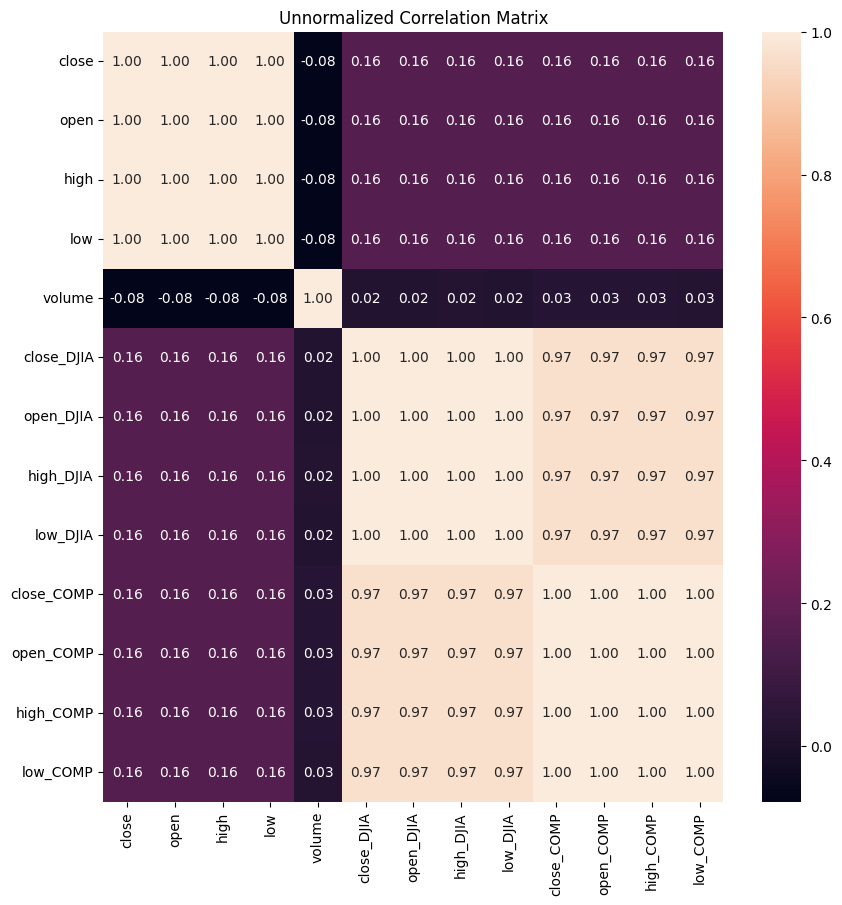
\includegraphics[width=\columnwidth]{figures/unnormCorr.png}
    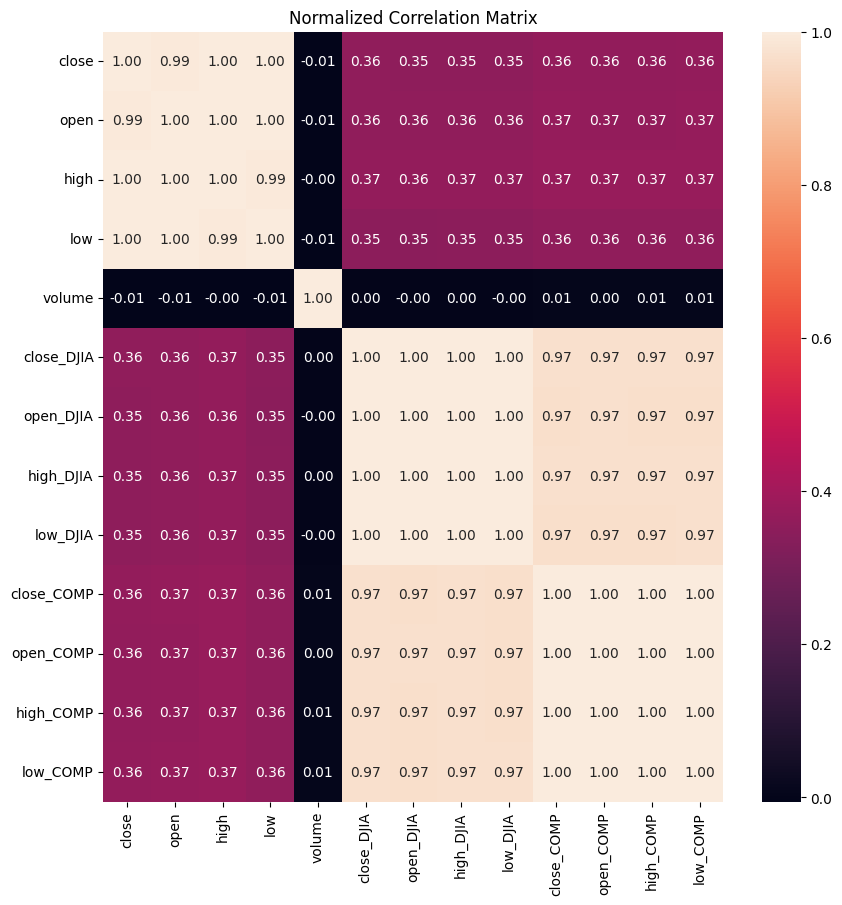
\includegraphics[width=\columnwidth]{figures/normCorr.png}
    \caption{Correlation of features in the dataset, unnormalized (left), and normalized by percent change from the start of the dataset (right).}
    \label{figure:correlations}
\end{figure*}

\begin{figure}
    \centering
    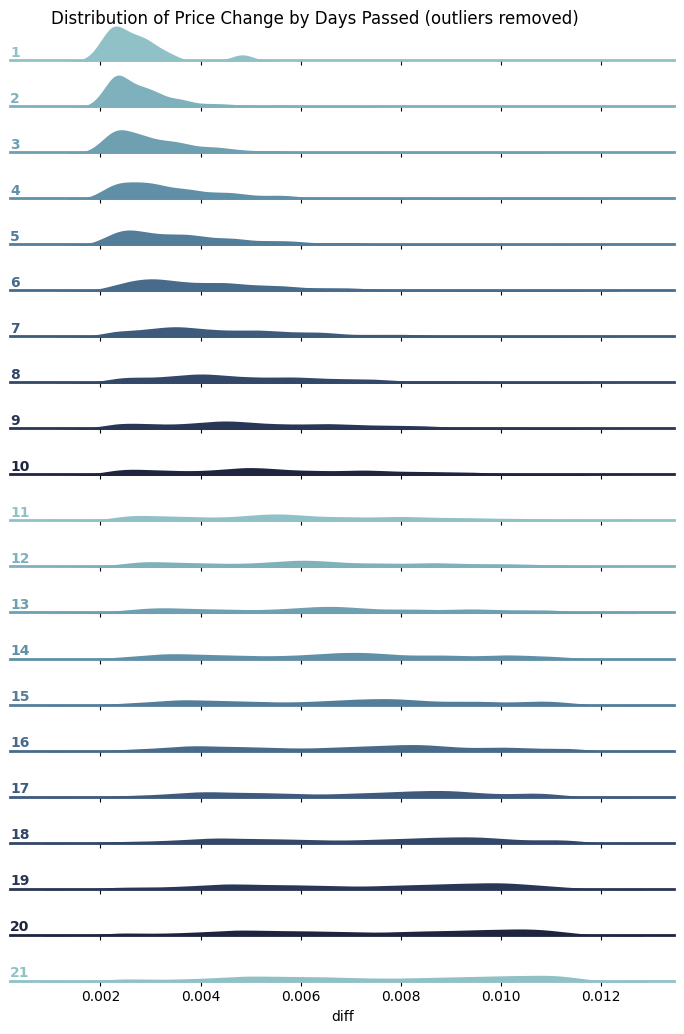
\includegraphics[width=\columnwidth]{figures/priceChangeByDays.png}
    \caption{Distribution of the change in stock price over the course of \it{N} days, averaged by stock.}
    \label{figure:priceChangeByDays}
\end{figure}

Some exploratory data analysis was conducted on the dataset to determine how useful certain features might be to machine learning models, and to gain an understanding of the difficulty of the problem. Figure \ref{figure:closeOverTime} shows the distribution of stock's closing prices by year. It can be seen that over time, the distribution becomes flatter as stock's prices increase over time. Despite the removal of outliers from the graph, it is also clearly visible that there is a large range of possible values for stock prices, and that it changes over time, so they must be normalized for models to perform properly. Figure \ref{figure:correlations} shows an example of this. It shows two correlation matrics, consisting of all features in the dataset, including the supplemental index data. When the data is unnormalized, the correlation between the index prices and the stock prices is much lower, as individual index prices are correlated against a wide range of stock prices. After normalizing both the stock prices and index prices by their percent change from the start of the dataset, the correlation is significantly increased, showing that the historical data for the indexes is likely to be useful in predicting stock prices. Additionally, the correlation matrices show that an individual stock's or index's prices are nearly perfectly correlated, and the prices of both indices are also nearly perfectly correlated. Figure \ref{figure:priceChangeByDays} shows the distribution of the change in stock price over the course of some number of days. While most stocks increase in price by an average of 0.2-0.4\% over the course of 1 day, this distribution becomes flatter and wider as more time passes, showcasing the difficulty of accurately forecasting stock price changes over longer time periods.

\subsection{Training}
Models were trained and evaluated by taking 6 months of stock data (126 days) and trying to predict the following one month of closing prices (21 days). These periods were collected as moving windows over the dataset, resulting in 1200232 training examples, 406244 validation examples, and 403731 test examples. While each model was given different input features and different preprocessing for those features, the labels were always preprocessed the same way in order to be able to compare the MSE loss of different models. The labels were normalized as the percent difference in price from the last day of the input data. Two main types of models were evaluated, neural networks and linear extrapolation (which did not require any training). Models were set up as JSON files containing the features to use, the functions to preprocess them with, and for neural networks, the layers comprising the network. Several different neural network architectures were tested, primarily feedforward neural networks, CNNs, and LSTMs.

Three different preprocessing functions were tested. The first function was min-max scaling over the input time period, where the minimum value was scaled to 0 and the maximum value was scaled to 1. The second function was equivalent to the the scaling for the labels, the percent difference in price from the last day of the input window (so the last day always had a value of zero). The last function was the percent change in price from the previous day. Each expression was implemented as a lazy-evaluated expression using the Polars dataframe library, and evaluated on the input window prior to being given to the model.

Models were trained for several epochs on random samples of 5\% of the training set, which were different for each epoch. Due to computational constraints arising from a lack of GPUs, training the models on the full training set each epoch took infeasible amounts of time. Models were trained with early stopping on the validation set, also a different random 5\% sample each epoch. If a model's loss on the validation sample failed to improve after 5 epochs, training would stop and the best model would be saved. Limited hyperparameter tuning was performed by hand, mostly only the number of layers and their parameters, such as the number of neurons per layer or the size of convolution kernels. Other hyperparameters such as the learning rate of the Adam optimizer were not modified.

\section{Experimental Results}

\begin{figure}
    \centering
    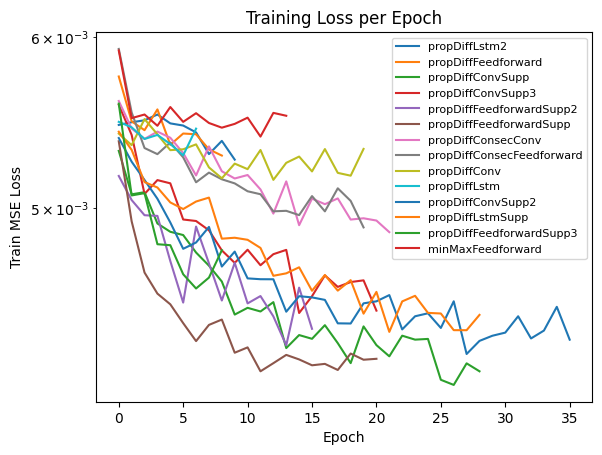
\includegraphics[width=\columnwidth]{figures/trainingLosses.png}
    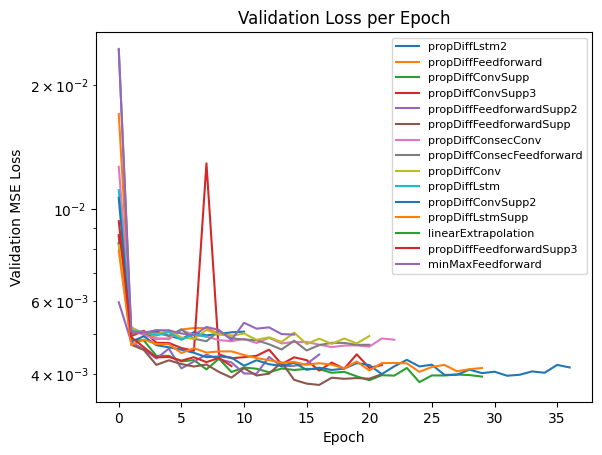
\includegraphics[width=\columnwidth]{figures/validationLosses.png}
    \caption{Training and validation MSE losses for each model.}
    \label{figure:trainValidLosses}
\end{figure}

\begin{figure}
    \centering
    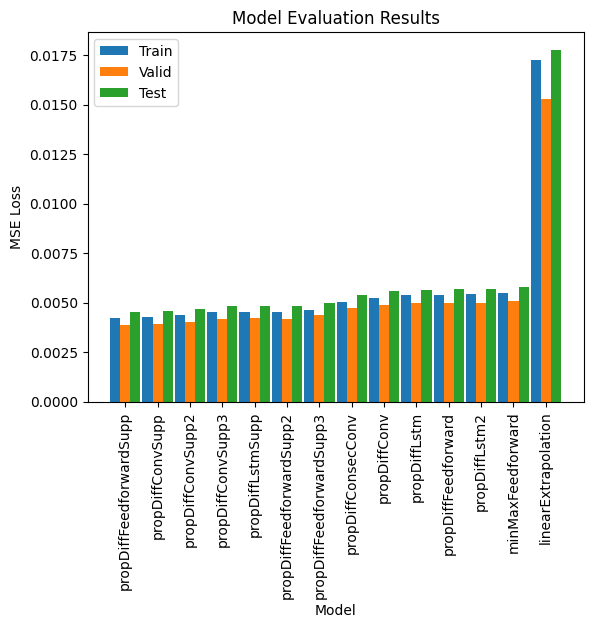
\includegraphics[width=\columnwidth]{figures/testLosses.png}
    \caption{MSE loss on the test set for each model.}
    \label{figure:testLosses}
\end{figure}

\begin{figure*}
    \centering
    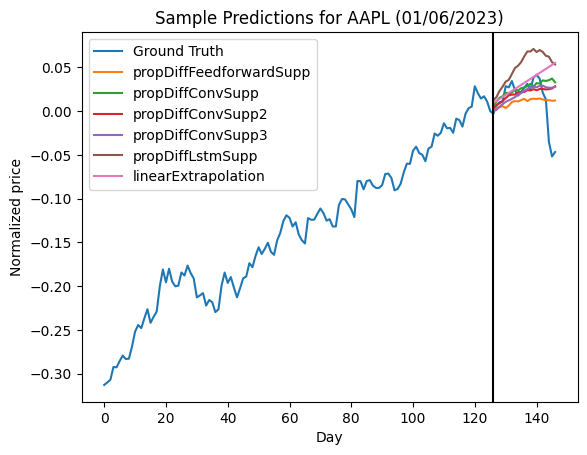
\includegraphics[width=\columnwidth]{figures/aaplSample.png}
    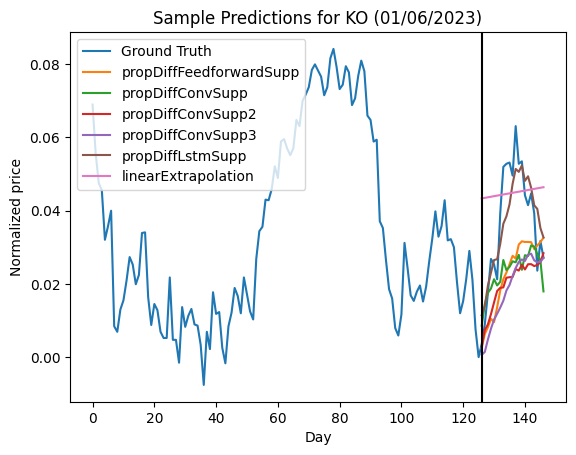
\includegraphics[width=\columnwidth]{figures/koSample.png}\\
    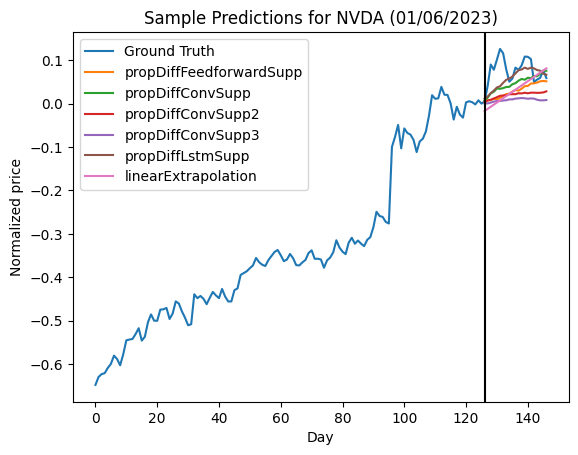
\includegraphics[width=\columnwidth]{figures/nvdaSample.png}
    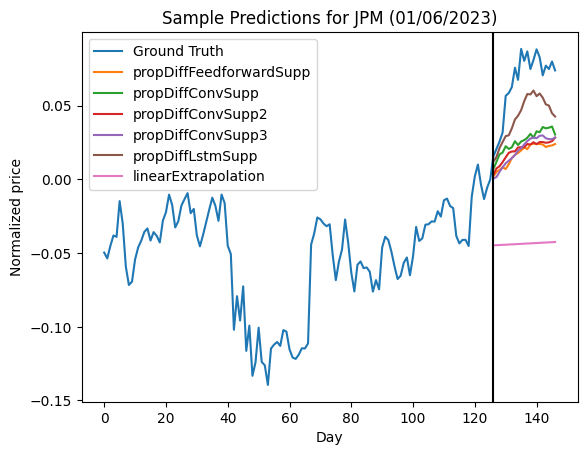
\includegraphics[width=\columnwidth]{figures/jpmSample.png}
    \caption{Example predictions for several different stocks from the test set. The 6 month input window for each example starts on 01/06/23, and 1 month of predictions is shown for each of the top 5 models and the baseline linear extrapolation.}
    \label{figure:examplePredictions}
\end{figure*}

Figure \ref{figure:trainValidLosses} shows the training and validation mean-squared error (MSE) loss of all the neural networks for each epoch. Most models that performed well took longer to train, whereas models that performed poorly tended to stop improving after very few epochs of training. Models that included supplemental data tended to both perform better and take longer to train, as they usually had significantly more parameters. Based on the training and validation losses, the best preprocessing function was the percent difference from the last day of the input data, though this may have just been a result of the fact that the labels were preprocessed in the same way. Limited experiments were performed with the other preprocessing functions after initial results showed poor performance. The spike in the validation MSE loss for one of the models shows problems inherent to the method of using random samples for validation, as varying difficulties in the random samples may have resulted in better models not being saved and vice versa.

Figure \ref{figure:testLosses} shows the MSE loss on the entire training, validation, and test sets for each neural network model, and the baseline linear extrapolation model. It can be seen that all models performed slightly better on the validation set, and slightly worse on the test set, implying that they all generalized to stocks they weren't trained on, but that the test consisted of more difficult stocks, and the validation set consisted of easier stocks. The linear extrapolation model had an MSE loss of 0.01777, which equates to an RMSE loss of 0.133, or approximately 13.3\% error in the predicted stock price. The best neural network model had an MSE loss of 0.0045, which equates to an RMSE loss of 0.0671, or approximately 6.71\% error in the predicted stock prices. The other neural network models performed somewhere in the middle, but even the worst had a 7.61\% error in the predicted stock price, which is significantly better than linear extrapolation. Additionally, models that included the supplemental index data always performed better than those that did not, showing the importance of considering the stock market as a whole when forecasting stock prices. The model that performed best was a simple feedforward neural network, though in general, CNNs performed better than other network architectures. LSTMs performed either really well, or really poorly, though the comparison may not be as fair due to limited hyperparameter tuning.

Figure \ref{figure:examplePredictions} shows example predictions on 4 different stocks from the test set, Apple Inc (AAPL), Coca-Cola Co (KO), NVIDIA Corp (NVDA), and JPMorgan Chase \& Co (JPM). The data for each sample prediction starts on January 6th 2023, and continues for 7 months, with the last month including the predictions from the top 5 neural network models and the linear extrapolation baseline. It can be seen that linear extrapolation performs poorly on all examples, but especially when the stock data is noisier and doesn't have a consistent trend. All the neural network models, aside from the LSTM, tend to have fairly similar predictions, generally predicting the trends in the stock price, though they perform worse when there are sudden spikes or dips in the stock price. The LSTM model tends to make really similar predictions in all 4 examples, with predicted price increasing quickly at the beginning and dropping the near the end of the month, though it also appears to be the most accurate on most of these examples. On KO specifically, the LSTM predicts the output almost perfectly, including the spikes in the middle of the predicted region, whereas the other models tend to only predict the start and end of the region well.

\section{Conclusion}
In conclusion, it seems like neural network models and more specifically, CNNs and LSTMs, are relatively good at forecasting stock prices, despite their noise and volatility, performing significantly better than linear extrapolation. The performance of the models also shows that stock index data can be very helpful for forecasting stock prices. The effect of different preprocessing methods might not have been entirely valid, given that the labels were not preprocessed in the same way as the input for certain models, leading to much more difficult training. In the future it might be worthwhile to experiment with different preprocessing for the labels, and converting them back to a consistent form for loss comparison. Additional future work might also include testing the performance of neural network models on smoothed data and labels, forecasting longer time periods, and comparing the performance with other better time-series forecasting methods, such as ARIMA. Experimenting with other neural network architectures and layers that tend to improve performance, such as dropout and batch normalization layers, may also prove worthwhile.

\clearpage
\nocite{*}
\bibliographystyle{ieeetran}
\bibliography{refs.bib}

\end{document}